\section{\textbf{Peterson Algorithm}}
% ------------------------------------------------------------------------ %
\subsection{Particular Case}
\par
In this experiment, the particular case we are trying to study is again mutual
exclusion where two threads try to use a shared resource.
\par
We are trying to do so in such a way that there is no starvation.
\par
% ------------------------------------------------------------------------ %
\subsection{Solution}
\par
During the lecture we discussed that Peterson algorithm takes the best of
other two algorithms (which we called the LockOne and the LockTwo) to create a
better one. The LockOne class that we discussed used an approach where mutual
exclusion was attempted using a flag which indicates that a given thread has the
intention of using a resource. We concluded that it satisfies the mutual
exclusion but it can potentially dead lock unless executions are not
interleaved.
\par
On the other hand, the LockTwo class achieved mutual exclusion by forcing the
threads let the other one execute first. However,  this approach also had dead
lock problems when one thread ran completely before the other one. So we observe
that both algorithms complement each other.
\par
 The Peterson algorithm combines these two methods to achieve a starvation-free
algorithm. It uses both the \textit{flags} approach and the
\textit{victimization} approach. 
\par
% ------------------------------------------------------------------------ %
\subsection{Experiment Description}
\par
 Now let's discuss how the proposed test case excersices the Peterson algorithm. 
 \par
 The test creates 2 threads that need to be coordinate in order to increment a
common counter. Both threads have to cooperate to increase this counter from 0
to 1024. Each of the threads will increase by one the counter 512 times. The
expected result is that regardless of the order in which each thread executes
the increment, at the end the counter must stay at 1024. If that is not the
case, then it means that mutual exclusion did not work.
\par
These are the details of the system we used to run the experiments:
\begin{enumerate}
\item Processor: Intel Core i5 @2.5 GHz. 2 Cores.
\item L2 Cache per Core: 256 KB
\item L3 Cache: 3 MB
\item System Memory: 16 GB
\end{enumerate}
% ------------------------------------------------------------------------ %
\subsection{Sample Results}
% ------------------------------------------------------------------------ %
\par
Figure \ref{fig:peterson} shows the output that we observed in the netbeans window:
\begin{figure}[h]
  \centering
  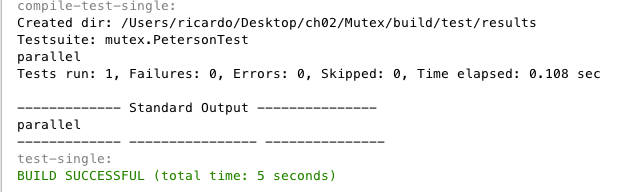
\includegraphics[width=13cm]{Peterson.png}
  \caption{Output of the junit test}
  \label{fig:peterson}
\end{figure}
\par
\begin{figure}[h]
  \centering
  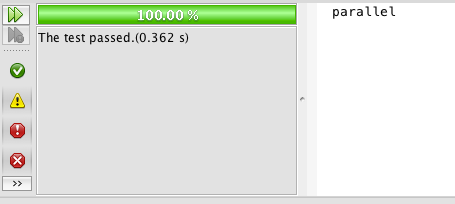
\includegraphics[width=10cm]{Peterson01.png}
  \caption{The Peterson test passed}
  \label{fig:peterson}
\end{figure}
% ------------------------------------------------------------------------ %
\subsection{Interpretation}
\par
The results in the proposed system were all OK. In all cases, the threads were
able to cooperate to increase the counter to 1024.
\par
One thing that is worth mentioning is that this algorihtm has a limitation. The
limitation is that it only works for two threads. In a later experiment we will
discover other algorithms that allow the coordination of more that two threads.
% ------------------------------------------------------------------------ %
